\documentclass[12pt]{article}
\usepackage[margin=1in]{geometry}
\usepackage{amsmath}
\usepackage{amssymb}
\usepackage{algorithmicx}
\usepackage{graphicx}
\usepackage{algorithm}
\usepackage{algpseudocode}
\usepackage[colorlinks=true, urlcolor = red, citecolor=blue, linkcolor=magenta]{hyperref}

\newcommand{\vect}[1]{\boldsymbol{#1}}
\newcommand{\Hel}{\hat{H}_{el}}
\newcommand{\R}{\mathbb{R}}
\newcommand{\Oh}{\mathcal{O}}
\newcommand{\norm}[1]{\left\lVert#1\right\rVert}

\begin{document}

\title{{\Large PS 10: Final Project -- Final Paper} \\ Automated Computation Of Molecular Properties \\ From First Principles}
\author{Alexander Lin \\ Supervised by Dr. Michael Mavros}

\maketitle

\section{Introduction}

In the world of chemistry, we are greatly interested in the ability to accurately solve the Schr\"odinger equation.  For molecular structures, solutions to the Schr\"odinger equation allow us to characterize many interesting properties, such as total energies, ionization potentials, and interatomic bond lengths, to name a few. 

However, since there do not exist exact, analytical solutions to many-body electron systems, the scientific community has resorted to computational approaches that make numerical approximations.  One of the most famous Schr\"odinger solvers that has been used throughout history is the Hartree-Fock algorithm \cite{szabo2012}.  By using a series of approximating methods -- such as Born-Oppenheimer, the single Slater Determinant, and the variational method -- Hartree-Fock allows us to compute an \emph{upperbound} to the true ground state energy $E$ of any given molecule, using nothing but the Cartesian coordinates and nuclear charges of its constituent atoms.   

In this project, we automate the implementation of Hartree-Fock for small molecules and derive interesting, experimentally-verified properties from first principles.  We begin by testing Hartree-Fock's ability to recover bond lengths of very simple inorganic molecules such as hydrogen fluoride and nitrogen gas.  Next, we evaluate how well the algorithm is able to calculate the total energy of various multi-electron atoms.  

Finally, we investigate the efficacy of Hartree-Fock in solving the Schr\"odinger equation for the GDB-13 dataset, an exhaustive enumeration of over 970 million organic and druglike molecules containing up to 13 atoms of cabon, nitrogen, oxygen, sulfur, and chlorine that are saturated with hydrogens \cite{blum2009}.  We focus on a subset of this dataset -- namely 59 small molecules with up to four non-hydrogen atoms from QM7b\footnote{Freely available at \url{http://quantum-machine.org/datasets/}.}, which was created to reduce the original dataset to a more manageable number of structures while maintaining the rich diversity of GDB-13 \cite{montavon2013}.  For each organic molecule, we compare a Hartree-Fock calculation of its total energy and first ionization potential to ground-truth values.  We also analyze trends within specific organic families such as alkanes and alkynes to show that Hartree-Fock can successfully recover these trends.  We conclude the analysis with experimental evidence that the asymptotic running time of Hartree-Fock is $\Oh(K^4)$, where $K$ is the number of orbitals considered by the algorithm for a given molecule.

The rest of this paper is organized as follows: Section 2 explains the mathematical theory behind the Hartree-Fock algorithm.  Section 3 details the process of implementing the algorithm, along with some technical specifications.  Section 4 presents the main results, thereby providing some evidence of the algorithm's utility.  And finally, Section 5 concludes the paper and touches on some potential future work.  

\section{Theory}

In this section, we heavily utilize the notation of \cite{sherrill2001} and \cite{szabo2012}.  We highly recommend interested readers to consult either of these comprehensive sources for additional information about Hartree-Fock theory.

\subsection{Initial Approximations}

Let us start with the Hamiltonian $\hat{H}$ and corresponding ground-state energy $E_{tot}$ for a multi-electron system.  The Hamiltonian can be characterized by five main components,
\begin{align}
\hat{H} = \hat{T}_N(\vect{R}) + \hat{T}_e(\vect{r}) + \hat{V}_{NN}(\vect{R}, \vect{Z}) + \hat{V}_{eN}(\vect{r}, \vect{R}, \vect{Z}) + \hat{V}_{ee}(\vect{r}),
\end{align}
where $\hat{T}_N, \hat{T}_e$ respectively describe the kinetic energies of the nuclei and electrons; and $\hat{V}_{NN}, \hat{V}_{eN}, \hat{V}_{ee}$ respectively describe the Coulombic potential energies of nucleus-nucleus repulsion, electron-nucleus attraction, and electron-electron attraction.  Here, $\vect{R} = \{\vect{R}_1, \ldots, \vect{R}_M\}$ and $\vect{r} = \{\vect{r}_1, \ldots, \vect{r}_N\}$ are matrices that hold three-dimensional coordinates for the $M$ nuclei and $N$ electrons of the molecule in question.  The vector $\vect{Z} = \{Z_1, \ldots, Z_M\}$ denotes the charges for the $M$ nuclei.  Note that $\vect{R}, \vect{Z}$ are inputs to the algorithm, whereas $\vect{r}$ is characterized by the wavefunction.  In general, we will use $\{i, j, k\}$ to index electrons and $\{A, B, C\}$ to index nuclei.     

The first approximation taken by Hartree-Fock is Born-Oppenheimer, which drops $\hat{T}_N$ from the Hamiltonian.  The other four terms can be expanded as,
\begin{align}
\hat{T}_e(\vect{r}) &= -\frac{1}{2} \sum_{i=1}^N \nabla_i^2 \label{t_e} , \\
\hat{V}_{NN}(\vect{R}, \vect{Z}) &= \sum_{A=1}^M \sum_{B > A}^M \frac{Z_A Z_B}{R_{AB}} \label{v_nn},\\
\hat{V}_{eN}(\vect{r}, \vect{R}, \vect{Z}) &=  - \sum_{A=1}^M \sum_{i=1}^N \frac{Z_{A}}{r_{Ai}} \label{v_en}, \\
\hat{V}_{ee}(\vect{r}) &= \sum_{i=1}^N \sum_{j > i}^N \frac{1}{r_{ij}} \label{v_ee}, 
\end{align}      
where $R_{AB} = \norm{\vect{R}_B - \vect{R}_A}_2$ is an internuclear distance, $r_{ij} = \norm{\vect{r}_j - \vect{r}_i}_2$ is an electron-electron distance, and $r_{Ai} = \norm{\vect{r}_i - \vect{r}_A}_2$ is an nucleus-electron distance.  One immediate observation from Equation \ref{v_nn} is that the operator $\hat{V}_{NN}$ has no dependence on electron coordinates $\vect{r}$; therefore, we can simply calculate this quantity at the beginning of the algorithm and leave it to the side.  It follows that the electronic Schr\"odinger equation may be simplified as 
\begin{align}
\hat{H}_{ele} \Psi(\vect{r}; \vect{R}, \vect{Z}) = \left[ \hat{T}_e(\vect{r}) + \hat{V}_{eN}(\vect{r}, \vect{R}, \vect{Z}) + \hat{V}_{ee}(\vect{r}) \right] \Psi(\vect{r}; \vect{R}, \vect{Z})= E_{ele} \Psi(\vect{r}; \vect{R}, \vect{Z}) \label{H_ele},
\end{align}
where the total energy of the multi-electron system $E_{tot} = E_{ele} + V_{NN}$ is the sum of the electronic and nuclear energies.

The antisymmetry principle states that for a system of fermions, the wavefunction must be antisymmetric with respect to changes in position \emph{and} spin of any two fermions \cite{sherrill2001}.  To satisfy this principle, we must introduce a new variable (i.e. the spin coordinate $\omega$) for each electron and define the wavefunction $\Psi$ in terms of $\vect{x} = \{\vect{x}_1, \ldots, \vect{x}_N\}$, where each $\vect{x}_i = \{\vect{r}_i, \omega_i\}$.  The following equation describes antisymmetry for any two electrons $i, j$,  
\begin{align}
\Psi(\vect{x}_1, \ldots, \vect{x}_i, \ldots, \vect{x}_j, \ldots, \vect{x}_N) = -\Psi(\vect{x}_1, \ldots, \vect{x}_j, \ldots, \vect{x}_i, \ldots, \vect{x}_N). \label{antisymm}
\end{align}  

We would like to express $\Psi$ as some aggregated function of single-electron, molecular wavefunctions $\chi_1, \ldots, \chi_n$ to make calculations easier.  Perhaps the most straightforward way to do this while satisfying Equation \ref{antisymm}  -- and its immediate corollary, the Pauli exclusion principle -- is to let $\Psi$ be a Slater determinant,
\begin{align}
\Psi(\vect{x}; \vect{R}, \vect{Z}) = \frac{1}{\sqrt{N!}} 
\begin{vmatrix}
\chi_1(\vect x_1) & \chi_2(\vect x_1)  & \cdots & \chi_N(\vect x_1) \\
\chi_1(\vect x_2) & \chi_2(\vect x_2)  & \cdots & \chi_N(\vect x_2) \\
\vdots & \vdots & \ddots & \vdots \\
\chi_1(\vect x_N) & \chi_2(\vect x_N) & \cdots & \chi_N(\vect x_N) 
\end{vmatrix}.
\end{align} 
That is, we assume $\Psi$ to be an anti-symmetric product-sum.  It is this assumption that makes Hartree-Fock a \emph{mean field approximation}, which means that each electron feels the average repulsive cloud of other electrons, but not the individual effects.  For this reason, the Hartree-Fock model fails to capture certain real-world phenomena, such as London dispersion, that occur between specific sets of electrons.  There exists an entire body of literature on post-Hartree-Fock methods for improving this approximation \cite{bartlett1994applications}.       

\subsection{Hartree-Fock Energy}
Following Sherrill's notation \cite{sherrill2001}, we can compactly re-express Equations \ref{t_e} and \ref{v_en} as a one-electron operator $\hat{h}$,
\begin{align}
\hat{T}_e(\vect{r}) + \hat{V}_{eN}(\vect{r}, \vect{R}, \vect{Z})  = \sum_{i} \left(-\frac{1}{2} \nabla_i^2 - \sum_A \frac{Z_A}{r_{iA}}\right) = \sum_{i} \hat{h}(i) ,
\end{align}
and Equation \ref{v_ee} as a two-electron operator $\hat{v}$,
\begin{align}
\hat{V}_{ee}(\vect{r}) = \sum_{i < j} \hat{v}(i, j) = \sum_{i < j} \frac{1}{r_{ij}}.
\end{align}
It follows that we can simply re-write the electronic Hamiltonian of Equation \ref{H_ele} as 
\begin{align}
\hat{H}_{ele}  = \sum_i \hat{h}(i) + \sum_{i < j}\hat{v}(i, j).
\end{align}

In finding the ground-state energy of a molecule, the goal of Hartree-Fock is to solve the following optimization problem, 
\begin{align}
E_{HF} = \min_{\Psi} E_{ele} = \min_{\Psi} \langle \Psi | \Hel | \Psi \rangle = \min_{\chi_1, \ldots, \chi_N} \sum_{i=1}^n \langle i | \hat{h} | i \rangle + \sum_{i=1}^n \sum_{j=i+1}^n [ i i | jj] - [ij | ji], 
\end{align}
where
\begin{align}
\langle i | \hat{h} | i \rangle &= \int_\R \chi_i^*(\vect x) \hat{h}(i) \chi_i (\vect x) d \vect x, \\
[ii | jj] &= \int_{\R^2} \chi_i^*(\vect x_1) \chi_i(\vect x_1) \hat{v}(i, j) \chi_j^*(\vect x_2) \chi_j(\vect x_2) d\vect x_1 \vect x_2, \\
[ij | ji] &= \int_{\R^2} \chi_i^*(\vect x_1) \chi_j(\vect x_1) \hat{v}(i, j) \chi_j^*(\vect x_2) \chi_i(\vect x_2) d\vect x_1 \vect x_2.
\end{align}

Working through Lagrange's method of undetermined multipliers for this optimization, as detailed in \cite{sherrill2000introduction}, we arrive at the eigenvalue problem,
\begin{align}
f(\vect{x}_1)\chi_i (\vect{x}_1) = \epsilon_i \chi_i(\vect{x}_1) \label{hf-eq},
\end{align}
where the Fock operator $f$ is defined by 
\begin{align}
f(\vect{x}_1) \chi_i (\vect{x}_1) &= h(\vect{x}_1) \chi_i (\vect{x}_1) + \sum_{j \neq i} \left[ \int  | \chi_j(\vect{x}_2) |^2 \frac{1}{r_{12}} d \vect{x}_2 \right] \chi_i (\vect{x}_1) \nonumber \\
&- \sum_{j \neq i} \left[ \int  \chi_j^* (\vect{x}_2) \chi_i(\vect{x}_2) \frac{1}{r_{12}} d \vect{x}_2 \right] \chi_j (\vect{x}_1),
\end{align}
and $\epsilon_i$ is the energy of molecular orbital $i$.  The operator involves the integration of complicated expressions, so to make things analytically tractable, we introduce a basis set of easy-to-integrate atomic orbitals $\tilde{\chi}_1, \ldots, \tilde{\chi}_K$.  Typically, $\tilde{\chi}_\mu$ is a linear combination of Gaussians whose coefficients have been optimized to fit Slater-type orbitals; we elaborate more on this in Section 3.  In doing so, we employ the variational principle -- another source of approximation.  

We now have that each molecular orbital $i$ is a linear combination of atomic orbitals (i.e. MO-LCAO method) with coefficients $C_{1i}, \ldots, C_{Ki}$, 
\begin{align}
\chi_i = \sum_{\mu = 1}^K C_{\mu i} \tilde{\chi}_\mu. 
\end{align}    

From this, we can rewrite Equation \ref{hf-eq} as the Hartree-Fock-Roothaan equations, 
\begin{align}
\sum_{\nu} F_{\mu \nu} C_{\nu i} = \epsilon_i \sum_{\nu} S_{\mu \nu} C_{\nu i} \label{hfr-eq},
\end{align}
where we have the more tractable integrals, 
\begin{align}
S_{\mu \nu} &= \int \tilde{\chi}_\mu^*(\vect{x}_1) \tilde{\chi}_\nu(\vect{x}_1) d \vect{x}_1 \label{overlap}, \\
F_{\mu \nu} &= \int \tilde{\chi}_\mu^*(\vect{x}_1) f(\vect{x}_1) \tilde{\chi}_\nu(\vect{x}_1) d \vect{x}_1 \label{fock}.
\end{align}

In matrix form, Equation \ref{hfr-eq} can be written as 
\begin{align}
\vect{F} \vect{C} = \vect{S} \vect{C} \vect{\epsilon} \label{hfr}
\end{align}

Equation \ref{hfr} is a peculiar eigenvalue equation, because $\vect{F}$ depends on $\vect{C}$ and vice-versa.  This means that both cannot be optimized simultaneously; instead, the Hartree-Fock algorithm must alternately update these two matrices until convergence.  

\subsection{Hartree-Fock Algorithm}

The Hartree-Fock algorithm \cite{szabo2012} can be divided into two main parts -- (1) integration and (2) iteration.  The integration part tends to dominate in terms of computation time.  

During the integration part, there are four main integrals of interest that need to be pre-computed.  The first is the overlap integral $S_{\mu \nu}$ for every pair of atomic orbitals $\mu, \nu$, as described by Equation \ref{overlap}.  The other three -- kinetic energy $T_{\mu \nu}$, nuclear-electron attraction $V_{\mu \nu}^\text{nucl}$, and electron-electron repulsion $[\mu \nu | \lambda \sigma]$ -- are involved in the Fock integral of Equation \ref{fock}.  Their expressions come straight from the operators -- as defined by Equations \ref{t_e}, \ref{v_en}, and \ref{v_ee} -- applied to the atomic basis functions,
\begin{align}
T_{\mu \nu} &= \int \tilde{\chi}^*_\mu(\vect{x}_1) \left[-\frac{1}{2} \nabla_1^2\right] \tilde{\chi}_\nu (\vect{x}_1) d \vect{r}_1,  \\
V_{\mu \nu}^\text{nucl} &= \int \tilde{\chi}^*_\mu(\vect{x}_1) \left[ - \sum_{A} \frac{Z_A}{r_{A1}} \right] \tilde{\chi}_\nu(\vect{x}_1) d\vect{r}_1, \\
[\mu \nu | \lambda \sigma]  &= \int \int \tilde{\chi}^*_\mu(\vect{x}_1) \tilde{\chi}_\nu(\vect{x}_1)  \left[\frac{1}{r_{12}}\right] \tilde{\chi}^*_\lambda(\vect{x}_2) \tilde{\chi}_\sigma(\vect{x}_2) d \vect{r}_1 \vect{r}_2.
\end{align}

After these integrals are computed, the algorithm proceeds by alternately changing $\vect{F}$ and $\vect{C}$.  A full description is given by \cite{szabo2012} and summarized in Algorithm \ref{alg}.  Note that this is the restricted Hartree-Fock procedure, which treats electrons as paired fermions and works for an even number of electrons.  

\begin{algorithm}
  \begin{algorithmic}[1]
  \State{\textbf{Input:} nuclear coords $\vect{R}$, charges $\vect{Z}$, atomic basis functions $\tilde{\chi}_\mu$, num of electrons $N$}
  \State{Compute nuclear-nuclear repulsion $V_{NN}$.}
  \State{Compute integrals $S_{\mu \nu}$, $T_{\mu \nu}$, $V_{\mu \nu}^\text{nucl}$, $[\mu \nu | \lambda \sigma]$}.  
  \State{Construct orthonormal basis transformation matrix $\vect{X}$ from $\vect{S}$ using canonical method.}
  \State{Initialize density matrix $\vect{P} = \vect{0}$.}
  \State{Initialize Fock matrix $F_{\mu \nu} = T_{\mu \nu} + V_{\mu \nu}^\text{nucl} $.}
  \While{$\vect{P}$ has not converged}
  \State{Calculate transformed Fock matrix $\vect{F}' = \vect{X}^T \vect{F} \vect{X}$.}
  \State{Diagonalize $\vect{F'}$ to get eigenvectors $\vect{C'}$ and eigenvalues $\vect{\epsilon}$.}
  \State{Calculate $\vect{C} = \vect{X} \vect{C'}$.}
  \State{Compute density matrix $P_{\mu \nu} = \sum_{i=1}^{N/2} C_{\mu i} C_{\nu i}$.}
  \State{Compute matrix $G_{\mu \nu} = \sum_{\lambda, \sigma} P_{\lambda \sigma} \left(2 \cdot [\mu \nu | \sigma \lambda] - [\mu \lambda | \sigma \nu] \right)$.}
  \State{Compute Fock matrix $F_{\mu \nu} = T_{\mu \nu} + V_{\mu \nu}^\text{nucl} + G_{\mu \nu}$.}
  \State{Compute electronic energy $E_{ele} = \sum_{\mu, \nu} P_{\mu \nu}  \cdot (T_{\mu \nu} + V_{\mu \nu}^\text{nucl} + F_{\mu \nu})$.}
  \EndWhile
  \State{Compute total energy $E_{tot} = E_{ele} + V_{NN}$.} 
  \State{\textbf{Output:} $E_{tot}, \vect{\epsilon}, \bold{F}, \bold{P}, \bold{T}, \bold{V}^\text{nucl}$}
  \end{algorithmic}
  \caption{Restricted Hartree-Fock} \label{alg}
\end{algorithm}

\section{Implementation}

Our implementation of Hartree-Fock follows Algorithm \ref{alg} and is written from scratch.  All code has been open-sourced and made available on GitHub\footnote{See \url{https://github.com/al5250/ps_10_final_project} for project code.}.  The algorithm is implemented using the Python programming language.  Almost everything involves the NumPy computing package, but we do use the SciPy computing package as well to calculate the Boys function \cite{helgaker2014molecular}, which is briefly needed in the integration of Gaussians.

\subsection{Atomic Basis Set -- STO-3G}    

The specific atomic orbital basis set that we choose to use is STO-3G, which was compiled by \cite{feller1996} and \cite{schuchardt2007}.  This is a minimal basis set; that is, a basis set that has the smallest possible size for reasonable results.  Each atom's orbital $\tilde{\chi}_\mu$ is a probability distribution function over possible locations $\vect{r}_i$ for a given electron $i$; it follows the form of a linear combination between three 3-dimensional Gaussians $g_1$, $g_2$, $g_3$ whose parameters $\alpha_{p \mu}$ and coefficients $d_{p \mu}$ have been pre-fit to a Slater-type orbital, 
\begin{align}
\tilde{\chi}_\mu(\vect{r}_i) \propto \sum_{p=1}^3 d_{p \mu} \cdot g_p(\vect{r}_i; \vect{R}_\mu, \alpha_{p \mu}). 
\end{align}       
Each Gaussian $g_p$ is centered at the nucleus $\vect{R}_\mu$ of atom $\mu$ and has an inverse-variance (sometimes also called "exponential") parameter $\alpha_{p \mu}$ that governs the spread of the distribution.  The Gaussian may take different forms depending on the orbital's azimuthal and magnetic quantum numbers, 
\begin{align}
g_p^{1s}(\vect{r}_i; \vect{R}_\mu, \alpha_{p \mu}) &= \left(\frac{8 \alpha_{p \mu}^3}{\pi^3}\right)^{1/4}  \exp(-\alpha_{p \mu} r_{i \mu}^2), \\
g_p^{2p_x}(\vect{r}_i; \vect{R}_\mu, \alpha_{p \mu}) &= \left(\frac{128 \alpha_{p \mu}^5}{\pi^3}\right)^{1/4}  (x_i - X_\mu) \exp(-\alpha_{p \mu} r_{i \mu}^2), \\
g_p^{2p_y}(\vect{r}_i; \vect{R}_\mu, \alpha_{p \mu}) &= \left(\frac{128 \alpha_{p \mu}^5}{\pi^3}\right)^{1/4}  (y_i - Y_\mu) \exp(-\alpha_{p \mu} r_{i \mu}^2), \\
g_p^{2p_z}(\vect{r}_i; \vect{R}_\mu, \alpha_{p \mu}) &= \left(\frac{128 \alpha_{p \mu}^5}{\pi^3}\right)^{1/4}  (z_i - Z_\mu) \exp(-\alpha_{p \mu} r_{i \mu}^2).
\end{align}
Note that in these equations, we implicitly unpack the vectors $\vect{r}_i = [x_i, y_i, z_i]^T$ and $\vect{R}_\mu = [X_\mu, Y_\mu, Z_\mu]^T$.  

There exist other basis sets STO-$P$G for $P = 1, 2, \ldots, 6$, but STO-3G is perhaps the most widely used.  Our code is general enough to apply to any STO-$P$G basis set. Also, there are more complicated basis sets such as 4-31G and 6-31G* \cite{schuchardt2007}, but these are outside the scope of this study.

\subsection{Integration} 

Since STO-3G atomic orbitals are fully characterized by Gaussians, we can apply rules for integration of Gaussian products to compute $S_{\mu \nu}$, $T_{\mu \nu}$, $V_{\mu \nu}^\text{nucl}$, and $[\mu \nu | \lambda \sigma]$.  The key insight is that integration of a product of two Gaussian probability distribution functions yields yet another Gaussian; thus, integration of any two Gaussians can be done in $\Oh(1)$-time.

For atomic orbitals with higher azimuthal quantum numbers (e.g. $p$-type orbitals), we must use recurrence relations to perform the integrations.  The mathematics become trickier and we defer the reader to \cite{helgaker2014molecular} for more information\footnote{The author of the text also has a set of accompanying slides at \url{http://folk.uio.no/helgaker/talks/SostrupIntegrals_10.pdf}}.  In particular, we follow the McMurchie-Davidson scheme in our code.  Since the results of Section 4 only involves small molecules, our implementation currently handles molecules containing elements up to the third row of the periodic table; some modifications will need to be made in order to handle $d$-type and $f$-type orbitals.         

The integration is also the rate-determining step of the Algorithm \ref{alg}.  Specifically, computing $[\mu \nu | \lambda \sigma]$ will take $\Oh(K^4)$-time, where $K$ is the number of atomic orbitals across all atoms in the molecule.  There are methods such as pre-screening electron-electron repulsion integrals \cite{helgaker2014molecular} that cut down the computation time; we implement pre-screening in our code, but for small molecules, we have found this modification to make little empirical difference.

\subsection{Code Description}

The main code is modularized in three Python files:  
\begin{itemize}
\item \texttt{utils.py} -- useful helper functions for parsing STO-3G basis set file, computing normalization coefficients and other useful quantities, etc.
\item \texttt{integrals.py} -- functions for calculating the four integrals in the integration step of the algorithm 
\item \texttt{hf.py} -- the main Hartree-Fock algorithm as detailed in Algorithm \ref{alg}; the primary wrapper function that covers all computation is called \texttt{hartree\_fock}.   
\end{itemize}              
There are also iPython notebooks in the repository that contain sample code for the experimental results detailed in Section 4.  Basis sets are found in the \texttt{basis\_sets} directory, while the data (including QM7b \cite{montavon2013}) is found in the \texttt{data} directory.      

\section{Results}

Using Hartree-Fock, we first reproduce some of the bond length results in \cite{szabo2012} for very small molecules.  Then, we calculate ground-state energy levels for all multi-electron atoms up to the third row in the periodic table and cross-reference the approximations with the true values in \cite{bunge1993roothaan}.  And finally, we provide a set of results on a dataset of 59 small organic molecules from QM7b \cite{montavon2013}.  All Hartree-Fock calculations are performed using the STO-3G basis set \cite{schuchardt2007}.  

\subsection{Equilibrium Bond Length}   
For diatomic molecules, the equilibrium bond length is the distance $r$ between the two atoms such that $E_{tot}$ is minimized.  For the molecules FH and N$_2$, we use our implementation of Algorithm \ref{alg} to plot the curve corresponding to $E_{tot}$ as a function of $r$ in Figure \ref{bond-len}.

\begin{figure}[h]
\begin{center}
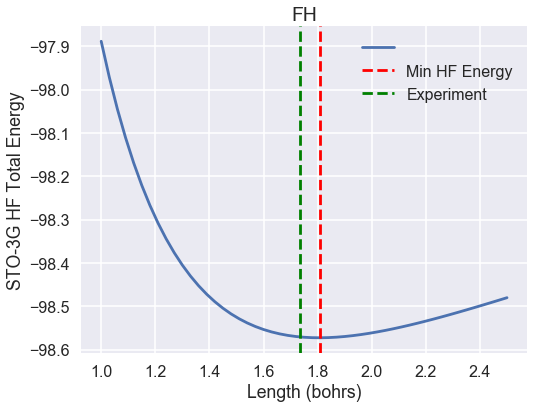
\includegraphics[scale=0.4]{img/bond-len-fh}
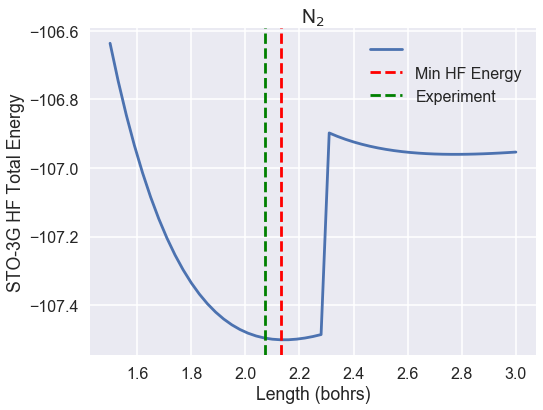
\includegraphics[scale=0.4]{img/bond-len-n2}
\end{center}
\caption{Total energy curves as a function of internuclear distance for diatomic molecules FH (left) and N$_2$ (right).  The dotted green line denotes the minimum of the blue curve, which was computed from first principles via Hartree-Fock.  The dotted red line denotes the true equilibrium bond length as found in experimental settings \cite{szabo2012}.  The errors are less than 10\% for both molecules.} \label{bond-len}
\end{figure} 

Notice that for N$_2$, we see a sudden jump in the Hartree-Fock energy at $r \approx 2.3$.  This is because the algorithm fails to converge to the true global minimum for the electronic energy $E_{ele}$ for $r \geq 2.3$; the algorithm could very well be identifying the 1st excited state, for example, instead of the ground state.

At this point, a natural question to ask if how limiting is the specific basis set we chose?  Could a different basis set (e.g. one more sophisticated than STO-3G) yield better results?  How much better would these results be?  For the sake of completeness, we show bond length results across different basis sets in Table \ref{bond-len-table}.  These results are taken from \cite{szabo2012}.  

\begin{table}
\begin{center}
\begin{tabular}{ c|cccc|c } 
 \hline 
 \hline
  & STO-3G & 4-31G & 6-31G$^*$ & Near-HF-limit & Experiment \\ 
 \hline
 FH & 1.807 & 1.742 & 1.722 & 1.696 & 1.733 \\ 
 N$_2$ & 2.143 & 2.050 & 2.039 & 2.013 & 2.074 \\ 
 \hline
 \hline
\end{tabular} 
\caption{Equilibrium bond length results derived using the Hartree-Fock algorithm for different basis sets.  All values are recorded in bohrs and taken from \cite{szabo2012}.  The results are not completely consistent with experimental data because of Hartree-Fock's inability to capture electron correlation effects \cite{bartlett1994applications}.} \label{bond-len-table}
\end{center}
\end{table}

\subsection{Atomic Energy}

Another use of Hartree-Fock is to calculate the total energy of a multi-electron atom.  However, given the \emph{restricted} nature of the algorithm that was implemented, we must input an even number of $N$ electrons.  Needless to say, not all neutral atoms have an even number of electrons.  Thus, we use the following scheme:

\begin{itemize}

\item If atom $X$ has an even number of $N$ electrons, then simply use Algorithm \ref{alg} to find $E_{tot}(X)$.  

\item If atom $X$ has an odd number of $N$ electrons, then $X^-$ must have an even number of $N + 1$ electrons.  Thus, we use Algorithm \ref{alg} to find $E_{tot}(X^-)$.  By Koopman's Theorem, the first ionization potential of an atom or molecule can be approximated by the negative of its highest occupied molecular orbital (HOMO) energy \cite{szabo2012}.  The HOMO energy is an output of Algorithm \ref{alg}, specifically $\epsilon_{(N+1) / 2}(X^-)$.  It follows that an approximation to $E_{tot}(X)$ is
\begin{align}
E_{tot}(X) \approx E_{tot}(X^-) - \epsilon_{(N+1) / 2}(X^-).
\end{align} 

\end{itemize}

Figure \ref{atom-energy} illustrates a comparison between the atomic energy as calculated by Hartree-Fock and a value that is essentially exact \cite{bunge1993roothaan} for atoms up to atomic number $Z = 18$.

\begin{figure}[h]
\begin{center}
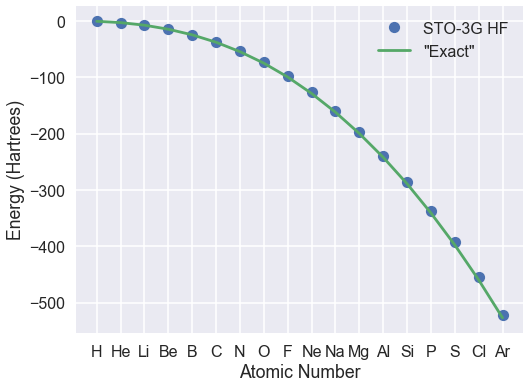
\includegraphics[scale=0.4]{img/atom-energy1}
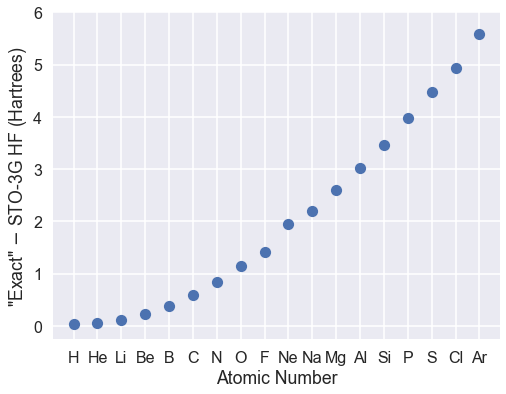
\includegraphics[scale=0.4]{img/atom-energy2}
\end{center}
\caption{A comparison of values calculated by a scheme based on Algorithm \ref{alg} and values taken from an essentially exact source \cite{bunge1993roothaan} for the total energy of a multi-electron atom (left).  The difference between the exact value and the calculated value seems to increase as the number of electrons increases, which is intuitive (right).} \label{atom-energy}
\end{figure} 

\subsection{Analysis of Small Organic Molecules}   

In this extended analysis, we report results for a small dataset of organic molecules containing up to four non-hydrogen atoms that are either carbon, nitrogen, or oxygen.  There are 59 molecules in total; the breakdown is 1 molecule with 1 non-hydrogen, 3 molecules with 2 non-hydrogens, 12 molecules with 3 non-hydrogens, and 43 molecules with 4 non-hydrogens.  

We begin by comparing differences between Algorithm \ref{alg}'s calculation of the total molecular energy and ground-truth "exact" values calculated using density functional theory that are provided by \cite{montavon2013}, the original source of the dataset.  The results are presented in Figure \ref{org-tot-energy}.  The mean absolute error is 7591 kcal per mol and the median absolute error is 7971 kcal per mol.  Notice that one of the organic molecules has an usually high error -- this is because the Hartree-Fock algorithm failed to converge within 100 iterations during the calculation of its total energy.  In general, the Hartree-Fock calculations are not very accurate, but the trends and patterns can be recovered. 

\begin{figure}[H]
\begin{center}
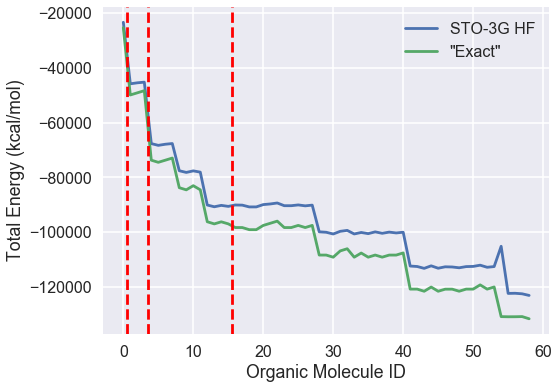
\includegraphics[scale=0.4]{img/org-tot-energy1}
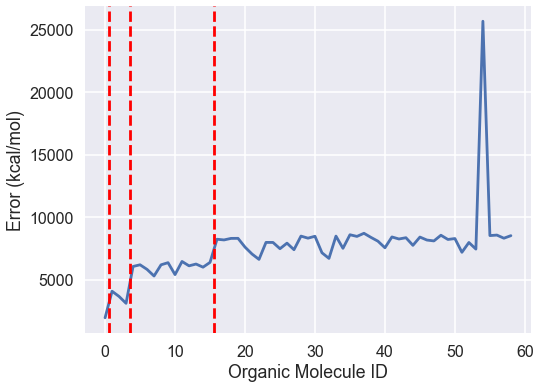
\includegraphics[scale=0.4]{img/org-tot-energy2}
\end{center}
\caption{A comparison of total energy values calculated by a scheme based on Algorithm \ref{alg} and values taken from an essentially exact source \cite{montavon2013} (left).  The dotted lines denote the delineations between 1 non-hydrogen, 2 non-hydrogen, 3 non-hydrogen, and 4 non-hydrogen structures.  As expected, the error increases as the complexity of the system increases (right).  Calculations for organic molecule \#54 failed to converge.} \label{org-tot-energy}
\end{figure} 

The most accurate set of results in this section are Hartree-Fock calculations of first ionization potentials for the organic molecules.  Given a molecule with $N$ electrons, we apply Koopman's Theorem to return $-\epsilon_{N / 2}$ as the ionization potential \cite{szabo2012}.  We compare our calculated values to those of \cite{montavon2013}.  The complete accuracy results are given in Figure \ref{ionize-energy}.  The mean absolute error is 3.6 eV with a mean absolute percentage error of 36\%.  The median absolute error is 2.5 eV with a mean absolute percentage error of 24\%.  The trends across certain organic families are also consistently maintained by the Hartree-Fock algorithm, which is shown in Figure \ref{ionize-fams}.    

Finally, we perform an analysis of the running time of the algorithm as a function of the number of atomic orbitals $K$.  In Section 2, we analytically derived this running time as $\Oh(K^4)$.  In Figure \ref{run-time}, we empirically show that this is the case.     

\begin{figure}[H]
\begin{center}
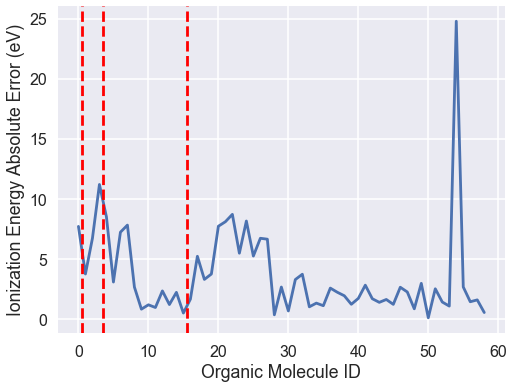
\includegraphics[scale=0.5]{img/ionize-energy}
\end{center}
\caption{The absolute error in first ionization potentials for different small organic molecules.  Ground truth is taken as density functional theory values reported in \cite{montavon2013}.  Again, the one outlier is a result of a failure of the algorithm to converge.} \label{ionize-energy}
\end{figure} 

\begin{figure}[H]
\begin{center}
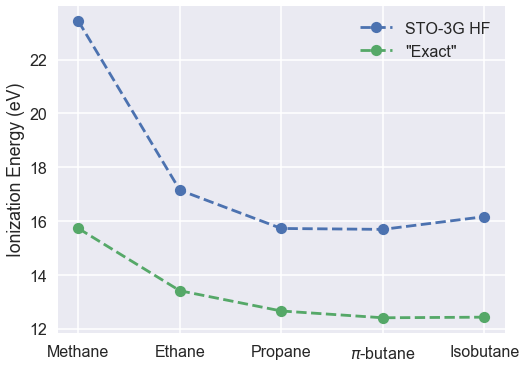
\includegraphics[scale=0.4]{img/alkanes}
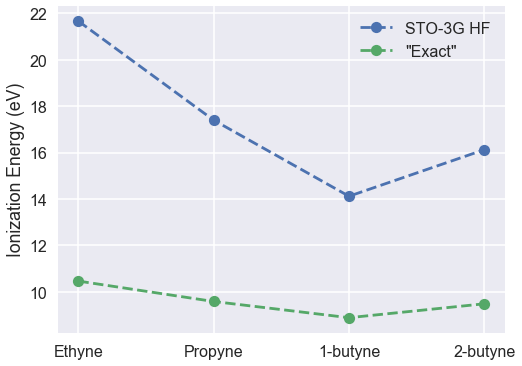
\includegraphics[scale=0.4]{img/alkynes}
\end{center}
\caption{Ionization energy calculations across different organic families -- alkanes (left) and alkynes (right).  The correct trends are maintained by the Hartree-Fock algorithm.} \label{ionize-fams}
\end{figure} 

\begin{figure}[H]
\begin{center}
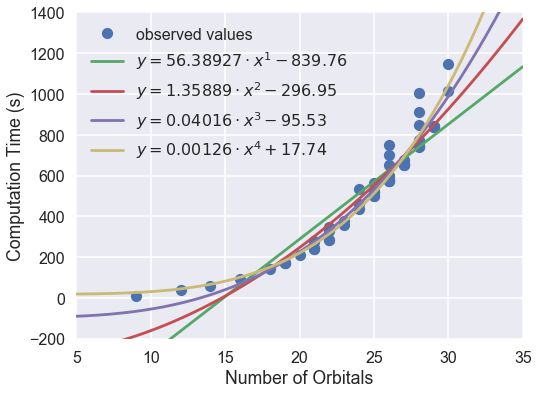
\includegraphics[scale=0.5]{img/run-time}
\end{center}
\caption{Fitting different polynomial curves to the running time of the algorithm versus number of atomic orbitals.  From this is analysis, it is clear that $\Oh(K^4)$ fits the best.} \label{run-time}
\end{figure} 

\section{Discussion and Conclusion}

In conclusion, we fully implemented the Hartree-Fock algorithm from scratch in Python.  Using this algorithm, we provided several results on calculating interesting properties, such as equilibrium bond length, total molecular energy, and first ionization potential.  In general, the Hartree-Fock algorithm provides useful calculations that are not exact, yet uncover interesting and accurate trends.  

In future work, there are several avenues for improvement.  For example, we can implement \emph{unrestricted} Hartree-Fock to directly calculate energies for molecules and atoms containing single-electron orbitals.  To improve accuracy, we can also try implementing other basis sets such as 4-31G or 6-31G*, which may give better results than the minimal STO-3G.  We can also explore implementation of post-Hartree-Fock methods such as coupled cluster, which takes electron correlation into account to improve algorithm accuracy.  However, it is well-known that the running time for coupled cluster may be as high as $\Oh(K^8)$ \cite{bartlett1994applications}, which means that we would need to take into account a tradeoff between speed and accuracy.  With improved accuracy, we can explore the calculation of other interesting molecular properties, such as atomization energy, that are hard to calculate accurately under the current Hartree-Fock paradigm.          

Finally, there is interest in seeing if other, non-physics-based approaches hold any promise in calculating these molecular energies accurately.  The $\Oh(K^4)$ running time of Hartree-Fock is certainly a limitation for larger molecules; perhaps statistics-based approaches such as machine learning could be useful in more efficiently calculating these values.  This is certainly an active area of research, especially with the success of deep learning neural networks in making progress towards many different regression problems \cite{montavon2012, montavon2013, rupp2012, mills2017}.  
  
\bibliographystyle{plain}
\bibliography{sources}

\end{document}